\documentclass{report}
%\usepackage{includegraphicx}
\usepackage{sydewkrpt}
\usepackage{longtable}
\usepackage{array}
\usepackage{ragged2e}
\usepackage{amsmath}
\usepackage{amssymb}
\DeclareMathOperator*{\argmin}{\arg\!\min}
\DeclareMathOperator*{\argmax}{\arg\!\max}
\newcolumntype{P}[1]{>{\RaggedRight\hspace{0pt}}p{#1}}

%%%%%%%%%%%%%%%%%%%%%%%%%%%%
%%%    Begin Document    %%%
%%%%%%%%%%%%%%%%%%%%%%%%%%%%
\begin{document}
\pagenumbering{roman}

\waterlootitle{SYDE 462: Spring Term Final Report}{
  Group 2: Relay \\
  Adaptive Traffic Control Framework
}{
  Alex Huras -- 20344660\\
  D. Scott Neil -- 20349210\\
  Myles Tan -- 20349217\\
  Riley Donelson -- 20342815\\
  }

\dotableofcontents

\newpage
\doublespacing
\pagenumbering{arabic}

\chapter{Background Information}
\setlength{\parindent}{1cm}

\newpage
\chapter{Engineering Design}

\section{Front End}

\section{Back End}

\section{Deep End}

\subsection{Learning in Relay}
\subsubsection{Design Parameter Updates}

Each agent within the system has multiple design parameters that will constantly update. With each cycle -- behaviour change -- predictions and estimations are made to recalculate these parameters. 
The following sections explain how these variables are learned and updated.

\subsubsection{Time Delay Estimation}
The first important parameter needed to calculate predictions is the time delay estimate between two agents. 
This can be thought of as the estimated time to travel from one intersection to a neighboring one. 
However, this is not a fixed time, so the delay is modeled using a gamma distribution, as discussed previously. 

The first step in performing this estimation, is determining which portion of the downstream signal is relevant – meaning what part of the signal should be considered for the estimation. 
This is required because it must ``match” the departing signal from the upstream intersection. 
To extract the downstream signal, an upstream sub-signal is first selected. It was determined that the most efficient way to do this is to this is to select the upstream departure signal created by the previous behaviour cycle. 
To ensure that events are not missed, the downstream signal is determined by time-shifting the upstream signal by the expected value of the previous time delay distribution, and a small buffer is added to each end.

After the two signals are extracted, the estimation process can be performed. 
Equation [time-delay-opt] outlines the optimization problem, using least squares. 
The goal of this optimization is to convolve the departure signal with a gamma distribution to best estimate the downstream arrival signal -- to minimize the difference between the real signal and estimated. 
The design parameters are: shape, location, scale, and gain. 
The first three are what control the parameters of the distribution and the last is a measure of the change in cars while traversing the road -- to capture the effect of cars turning onto or off of the road on side streets.

Below, in Figure \ref{fig:time-delay-est}, an example estimate is performed. 
Two signals are provided (departure is pre-calculated within the agent and not shown here), trimmed, and then the optimization procedure is executed. 
The resulting distribution is overlaid on the downstream signal and estimated time delay gamma plotted above.

\begin{figure}[htbp!]
  \begin{centering}
    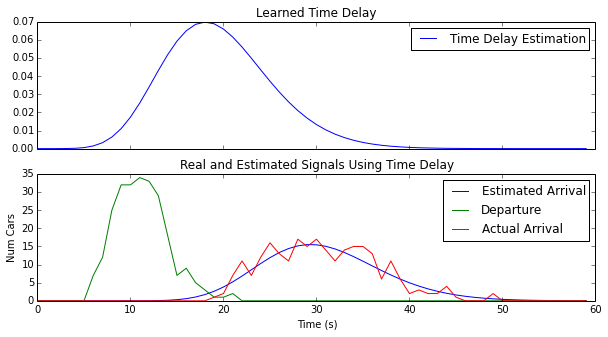
\includegraphics[scale=0.75]{figures/time-delay-est.png}
    \caption{Example time delay estimation.}
    \label{fig:time-delay-est}
  \end{centering}
\end{figure}


\subsubsection{Updating Intra-Agent Behaviour Graphs}
The second important piece in generating signal predictions is learning the intra-agent graph probabilities. 
These represent the likelihood of a signal to travel along this edge during the executed behaviours cycle.

\paragraph{Behaviour Probability Matrix (BPM)}
Figure \ref{fig:BPM-example} provides a visualization of this to help parse this idea. 
The matrix represents how these edge probabilities are used within the system; in the matrix, departing nodes are along the columns and entering along the rows -- $p_{02}$ would represent entering node 0 and exiting node 2. 
It is seen in the diagram that an event occurring at node 0 has a 60% likelihood of exiting node 2, for this behaviour.
 It is important to not that edges that are not traversable will always have a probability of 0. 
Essentially, this probability matrix is used to split an entering signal into components, to then be combined with other estimates in a departing signal. 
This estimated signal is then used in combination with the time delay estimation to predict expected traffic, which will be discussed further in the following section.

\begin{figure}[htbp!]
  \begin{centering}
    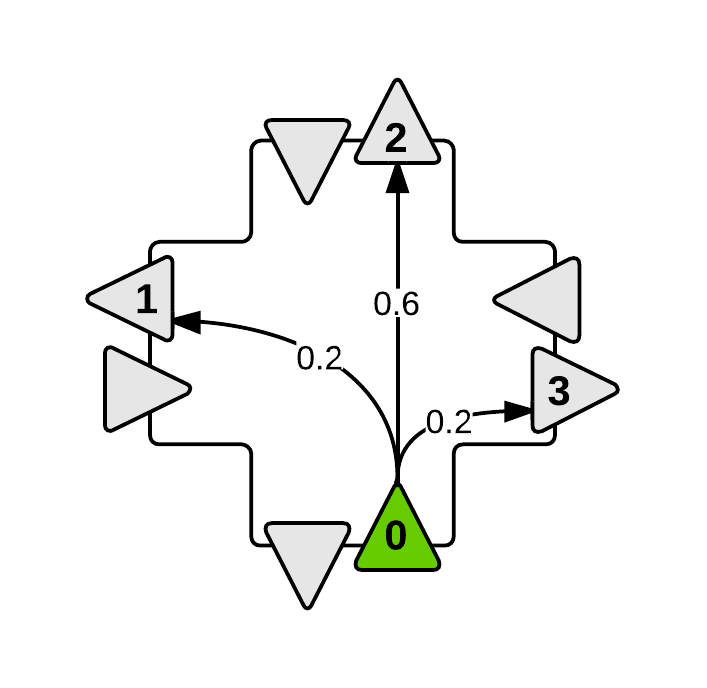
\includegraphics[scale=0.3]{figures/BPM-example.png}
    \caption{Example intra-agent edge probabilities for node 0.}
    \label{fig:BPM-example}
  \end{centering}
\end{figure}


\[
{BPM} =
    \begin{bmatrix}
    p_{00} & p_{01} & p_{02} & p_{03} \\
    p_{10} & p_{11} & p_{12} & p_{13} \\
p_{20} & p_{21} & p_{22} & p_{23} \\
p_{30} & p_{31} & p_{32} & p_{33} \\
    \end{bmatrix}
\]

\paragraph{Learning Probabilities}

\paragraph{Updating BPMs}
After the optimization procedure has arrived at a solution, the existing BPM must be updated. 
It would be unwise to directly use the newly calculated BPM as temporary inhibitors to traffic flow, such as accidents, can greatly skew results. 
Therefore, a learning parameter is used to update existing probabilities, seen in Equation \ref{eqn:BPM-update}. 
This can be tuned, on an agent-by-agent basis, to alter how quickly these values are modified and adapt – an average of the two values is a good starting point, to enable quick transitions, while remaining relatively stable. 
In \ref{eqn:BPM-update}, $i$ represents the agents ID and $BPM_{est}^{i}$ is the newly estimated behaviour probability matrix for that agent.

\begin{equation}
    BPM_{new}^{i} = \alpha^{i} \times BPM_{old}^{i} + (1 - \alpha^{i}) \times BPM_{est}^{i}
    \label{eqn:BPM-update}
\end{equation}

\newpage
\chapter{Design Testing and Validation}

\section{Front End}

\section{Back End}

\section{Deep End}

\newpage
\chapter{Recommended Design Modifications}

\newpage
\chapter{Timeline and Project Management}

\newpage
\section{Conclusion}

\newpage
\addcontentsline{toc}{section}{References}

\bibliographystyle{IEEEtran}

\bibliography{bib}

\end{document}
